\documentclass[tikz,border=5pt]{standalone}
\usepackage{tikz}
\usetikzlibrary{positioning,arrows.meta,shapes.geometric,fit,backgrounds}

\begin{document}
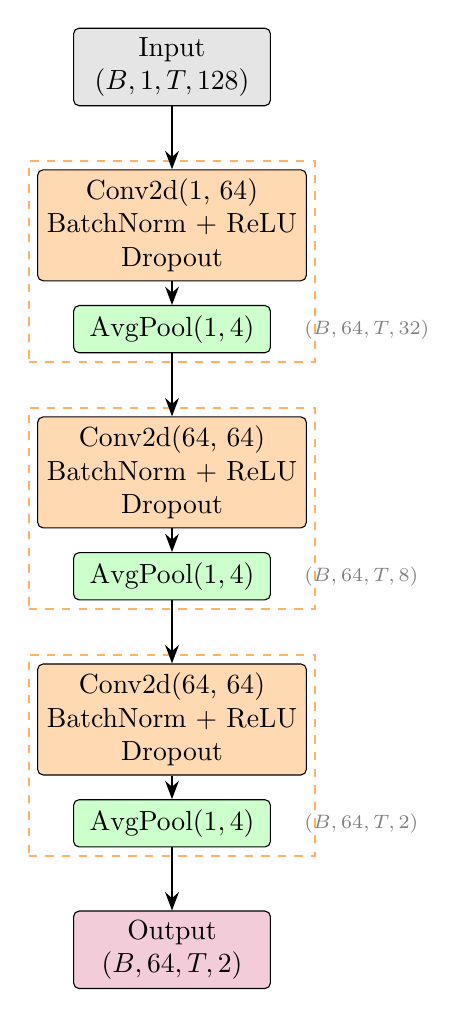
\begin{tikzpicture}[
    node distance=0.8cm,
    block/.style={rectangle, draw, fill=blue!20, minimum width=2.5cm, minimum height=0.8cm, align=center, rounded corners=2pt},
    convblock/.style={rectangle, draw, fill=orange!30, minimum width=2.5cm, minimum height=1.2cm, align=center, rounded corners=2pt},
    poolblock/.style={rectangle, draw, fill=green!20, minimum width=2.5cm, minimum height=0.6cm, align=center, rounded corners=2pt},
    arrow/.style={-{Stealth}, thick},
    label/.style={font=\scriptsize, text=gray}
]

% Input
\node[block, fill=gray!20] (input) {Input\\$(B, 1, T, 128)$};

% Conv Block 1
\node[convblock, below=of input] (conv1) {Conv2d(1, 64)\\BatchNorm + ReLU\\Dropout};
\node[poolblock, below=0.3cm of conv1] (pool1) {AvgPool$(1, 4)$};

% Conv Block 2
\node[convblock, below=of pool1] (conv2) {Conv2d(64, 64)\\BatchNorm + ReLU\\Dropout};
\node[poolblock, below=0.3cm of conv2] (pool2) {AvgPool$(1, 4)$};

% Conv Block 3
\node[convblock, below=of pool2] (conv3) {Conv2d(64, 64)\\BatchNorm + ReLU\\Dropout};
\node[poolblock, below=0.3cm of conv3] (pool3) {AvgPool$(1, 4)$};

% Output
\node[block, fill=purple!20, below=of pool3] (output) {Output\\$(B, 64, T, 2)$};

% Arrows
\draw[arrow] (input) -- (conv1);
\draw[arrow] (conv1) -- (pool1);
\draw[arrow] (pool1) -- (conv2);
\draw[arrow] (conv2) -- (pool2);
\draw[arrow] (pool2) -- (conv3);
\draw[arrow] (conv3) -- (pool3);
\draw[arrow] (pool3) -- (output);

% Dimension labels
\node[label, right=0.3cm of pool1] {$(B, 64, T, 32)$};
\node[label, right=0.3cm of pool2] {$(B, 64, T, 8)$};
\node[label, right=0.3cm of pool3] {$(B, 64, T, 2)$};

% Block groupings
\begin{scope}[on background layer]
    \node[draw=orange!60, dashed, thick, fit=(conv1)(pool1), inner sep=3pt, label={[font=\scriptsize]left:Block 1}] {};
    \node[draw=orange!60, dashed, thick, fit=(conv2)(pool2), inner sep=3pt, label={[font=\scriptsize]left:Block 2}] {};
    \node[draw=orange!60, dashed, thick, fit=(conv3)(pool3), inner sep=3pt, label={[font=\scriptsize]left:Block 3}] {};
\end{scope}

\end{tikzpicture}
\end{document}
